\documentclass[11pt, a4paper]{article}
\usepackage[margin=2.5cm]{geometry}
\usepackage{amsmath}
\usepackage{graphicx}
\usepackage[hidelinks]{hyperref}
\usepackage{caption}
\usepackage{subcaption}
\usepackage{listings}
\usepackage{xcolor}
\definecolor{codegray}{rgb}{0.95,0.95,0.95}
\lstset{
  backgroundcolor=\color{codegray},
  basicstyle=\ttfamily\footnotesize,
  frame=single,
  breaklines=true,
  postbreak=\mbox{\textcolor{red}{$\hookrightarrow$}\space},
  numbers=left,
  numberstyle=\tiny,
  numbersep=5pt,
  captionpos=b
}
\title{Drug Diffusion in Biological Tissues: Mathematical Analysis and Numerical Simulation}
\author{Julien Fernandes -- \href{mailto:julien.fernandes@edu.devinci.fr}{julien.fernandes@edu.devinci.fr}}
\date{26 May 2025}
\begin{document}

\maketitle
\begin{center}
\fbox{
  \begin{minipage}{0.85\textwidth}
    \centering
    \textbf{Institution:} Dorset College, Dublin \\
    \textbf{Course:} Partial Differential Equations \\
    \textbf{Instructor:} Solenn Hughes -- \href{mailto:solenn@dorset.ie}{solenn@dorset.ie} \\
  \end{minipage}
}
\end{center}

\vspace{1cm}
\noindent\textbf{Project Repository:} \href{https://github.com/julien7518/Drug-Diffusion-in-Biological-Tissues}{github.com/julien7518/Drug-Diffusion-in-Biological-Tissues}
\hypersetup{linktoc=all}
\tableofcontents
\newpage

\section{Introduction}
Drug delivery is a fundamental process in medicine, especially when it comes to treating diseases in specific tissues.
When a drug is administered, it often needs to spread through biological tissues to reach the targeted area.
Understanding how drugs move and spread inside tissues is important for improving treatments, avoiding side effects, and designing better drug delivery systems.
This report focuses on the mathematical modeling of drug diffusion in biological tissues. We will explore a well-known partial differential equation called the diffusion equation, analyze it theoretically, and solve it using numerical methods.
Our goal is to understand how this equation helps us describe the movement of drugs in 2D tissues and to simulate this process using Python.

\section{Literature Review and Context}

\subsection{Origin of the Diffusion Equation}
The diffusion equation is a type of partial differential equation (PDE) that describes how a quantity such as heat, particles, or drugs spreads over time.
It was first studied in detail by Joseph Fourier in the early 19th century in the context of heat transfer.
Fourier introduced the concept of using mathematical equations to describe how heat moves through solid bodies.
Later, Adolf Fick applied similar ideas to the movement of particles in liquids and gases. Fick’s laws of diffusion, published in 1855, are still used today to describe molecular diffusion in biological systems.

The standard form of the diffusion equation in two dimensions is:
\[
\frac{\partial u}{\partial t} = D \left( \frac{\partial^2 u}{\partial x^2} + \frac{\partial^2 u}{\partial y^2} \right)
\]
where \( u(x, y, t) \) is the concentration of the substance at position \((x, y)\) and time \(t\), and \(D\) is the diffusion coefficient. This equation can be extended to include anisotropy and reaction terms to better model complex situations in biology.

\subsection{Biomedical Applications}
In medicine and biology, diffusion is important for understanding how substances like oxygen, nutrients, and drugs move through tissues.
For example, when a drug is injected or delivered through the skin, it must diffuse through layers of tissue to reach its target.
This process is influenced by the properties of the tissue, such as density, porosity, and anisotropy (when diffusion is faster in one direction than another).

Drug diffusion models are used in pharmacokinetics to study how drugs move in the body, how long they stay active, and where they accumulate.
These models help in the design of drug delivery systems like transdermal patches, implants, or controlled-release capsules.
They are also important in cancer therapy, where accurate diffusion models can help predict how chemotherapy drugs spread in tumor tissues.

\subsection{Key Works and References}
Many researchers have contributed to the modeling of drug diffusion. While classical works such as J. Crank’s book “The Mathematics of Diffusion” and “Mathematical Physiology” by Keener and Sneyd provide deep mathematical understanding, they can be quite technical. For more accessible information, we recommend the following online sources:

\begin{itemize}
  \item ScienceDirect: \url{https://www.sciencedirect.com/}
  \item SpringerLink: \url{https://link.springer.com/}
  \item PubMed: \url{https://pubmed.ncbi.nlm.nih.gov/}
  \item Article: “Mathematical modeling of drug delivery” - \url{https://www.ncbi.nlm.nih.gov/pmc/articles/PMC5763252/}
  \item Review: “Drug transport in tumor tissue” - \url{https://www.ncbi.nlm.nih.gov/pmc/articles/PMC7491225/}
  \item General overview: Wikipedia - \url{https://en.wikipedia.org/wiki/Diffusion}
\end{itemize}

\section{Theoretical Exploration}

\subsection{Equation Classification}
The diffusion equation used in this project is a second-order partial differential equation (PDE) that is classified as a parabolic equation. Parabolic PDEs describe processes that involve time evolution with smoothing or spreading behavior, such as heat conduction or chemical diffusion. In our case, the diffusion equation models the change in drug concentration over time in a 2D spatial domain.

Parabolic equations typically have one time derivative and second-order spatial derivatives. They are known to generate solutions that are continuous and smooth as time increases, even if the initial conditions are not. This makes them suitable for modeling physical processes where the substance gradually spreads out.

\subsection{Mathematical Structure}
The general 2D diffusion equation without reaction terms is:
\[
\frac{\partial u}{\partial t} = D_x \frac{\partial^2 u}{\partial x^2} + D_y \frac{\partial^2 u}{\partial y^2}
\]
where:
\begin{itemize}
    \item \( u(x, y, t) \) is the drug concentration at time \(t\),
    \item \( D_x \) and \( D_y \) are the diffusion coefficients in the \(x\) and \(y\) directions.
\end{itemize}

When \( D_x \neq D_y \), the diffusion is anisotropic, meaning the drug spreads at different speeds depending on direction. This is common in biological tissues where fibers or structures can guide the movement of molecules.

If we add a reaction term to model absorption or decay of the drug, we get:
\[
\frac{\partial u}{\partial t} = D_x \frac{\partial^2 u}{\partial x^2} + D_y \frac{\partial^2 u}{\partial y^2} - \lambda u
\]
where \( \lambda \) is the reaction rate (e.g., drug being absorbed or metabolized).

The diffusion equation is linear, which means we can use superposition to build more complex solutions. It also satisfies conservation of mass in the absence of sources or sinks.

% --- Begin replacement ---
\subsection{Simplified Analytical Solution}
To better understand the behavior of the diffusion equation, we solve a simplified version analytically. We assume:
\begin{itemize}
    \item Isotropic diffusion: \( D_x = D_y = D \)
    \item No reaction: \( \lambda = 0 \)
    \item Infinite domain in 2D
    \item Initial condition: a point source at the origin, modeled by a Dirac delta function: \( u(x, y, 0) = \delta(x) \delta(y) \)
\end{itemize}

The 2D diffusion equation becomes:
\[
\frac{\partial u}{\partial t} = D \left( \frac{\partial^2 u}{\partial x^2} + \frac{\partial^2 u}{\partial y^2} \right)
\]

This is a linear PDE, and we can solve it using the 2D Fourier transform method. Taking the Fourier transform in both spatial variables, we obtain:
\[
\mathcal{F}[u](k_x, k_y, t) = \hat{u}(k_x, k_y, t)
\]
\[
\frac{\partial \hat{u}}{\partial t} = -D (k_x^2 + k_y^2) \hat{u}
\]

This is an ordinary differential equation (ODE) in time. Solving it gives:
\[
\hat{u}(k_x, k_y, t) = \hat{u}(k_x, k_y, 0) \cdot \exp\left( -D (k_x^2 + k_y^2) t \right)
\]

Because the initial condition is a delta function, its Fourier transform is constant:
\[
\hat{u}(k_x, k_y, 0) = 1
\]

Thus,
\[
\hat{u}(k_x, k_y, t) = \exp\left( -D (k_x^2 + k_y^2) t \right)
\]

Taking the inverse Fourier transform, we recover the spatial solution:
\[
u(x, y, t) = \frac{1}{4\pi D t} \exp\left( -\frac{x^2 + y^2}{4Dt} \right)
\]

This is a Gaussian function with spreading radius increasing over time. It shows that the concentration becomes more spread out and less intense at the origin.

\begin{figure}[h!]
  \centering
  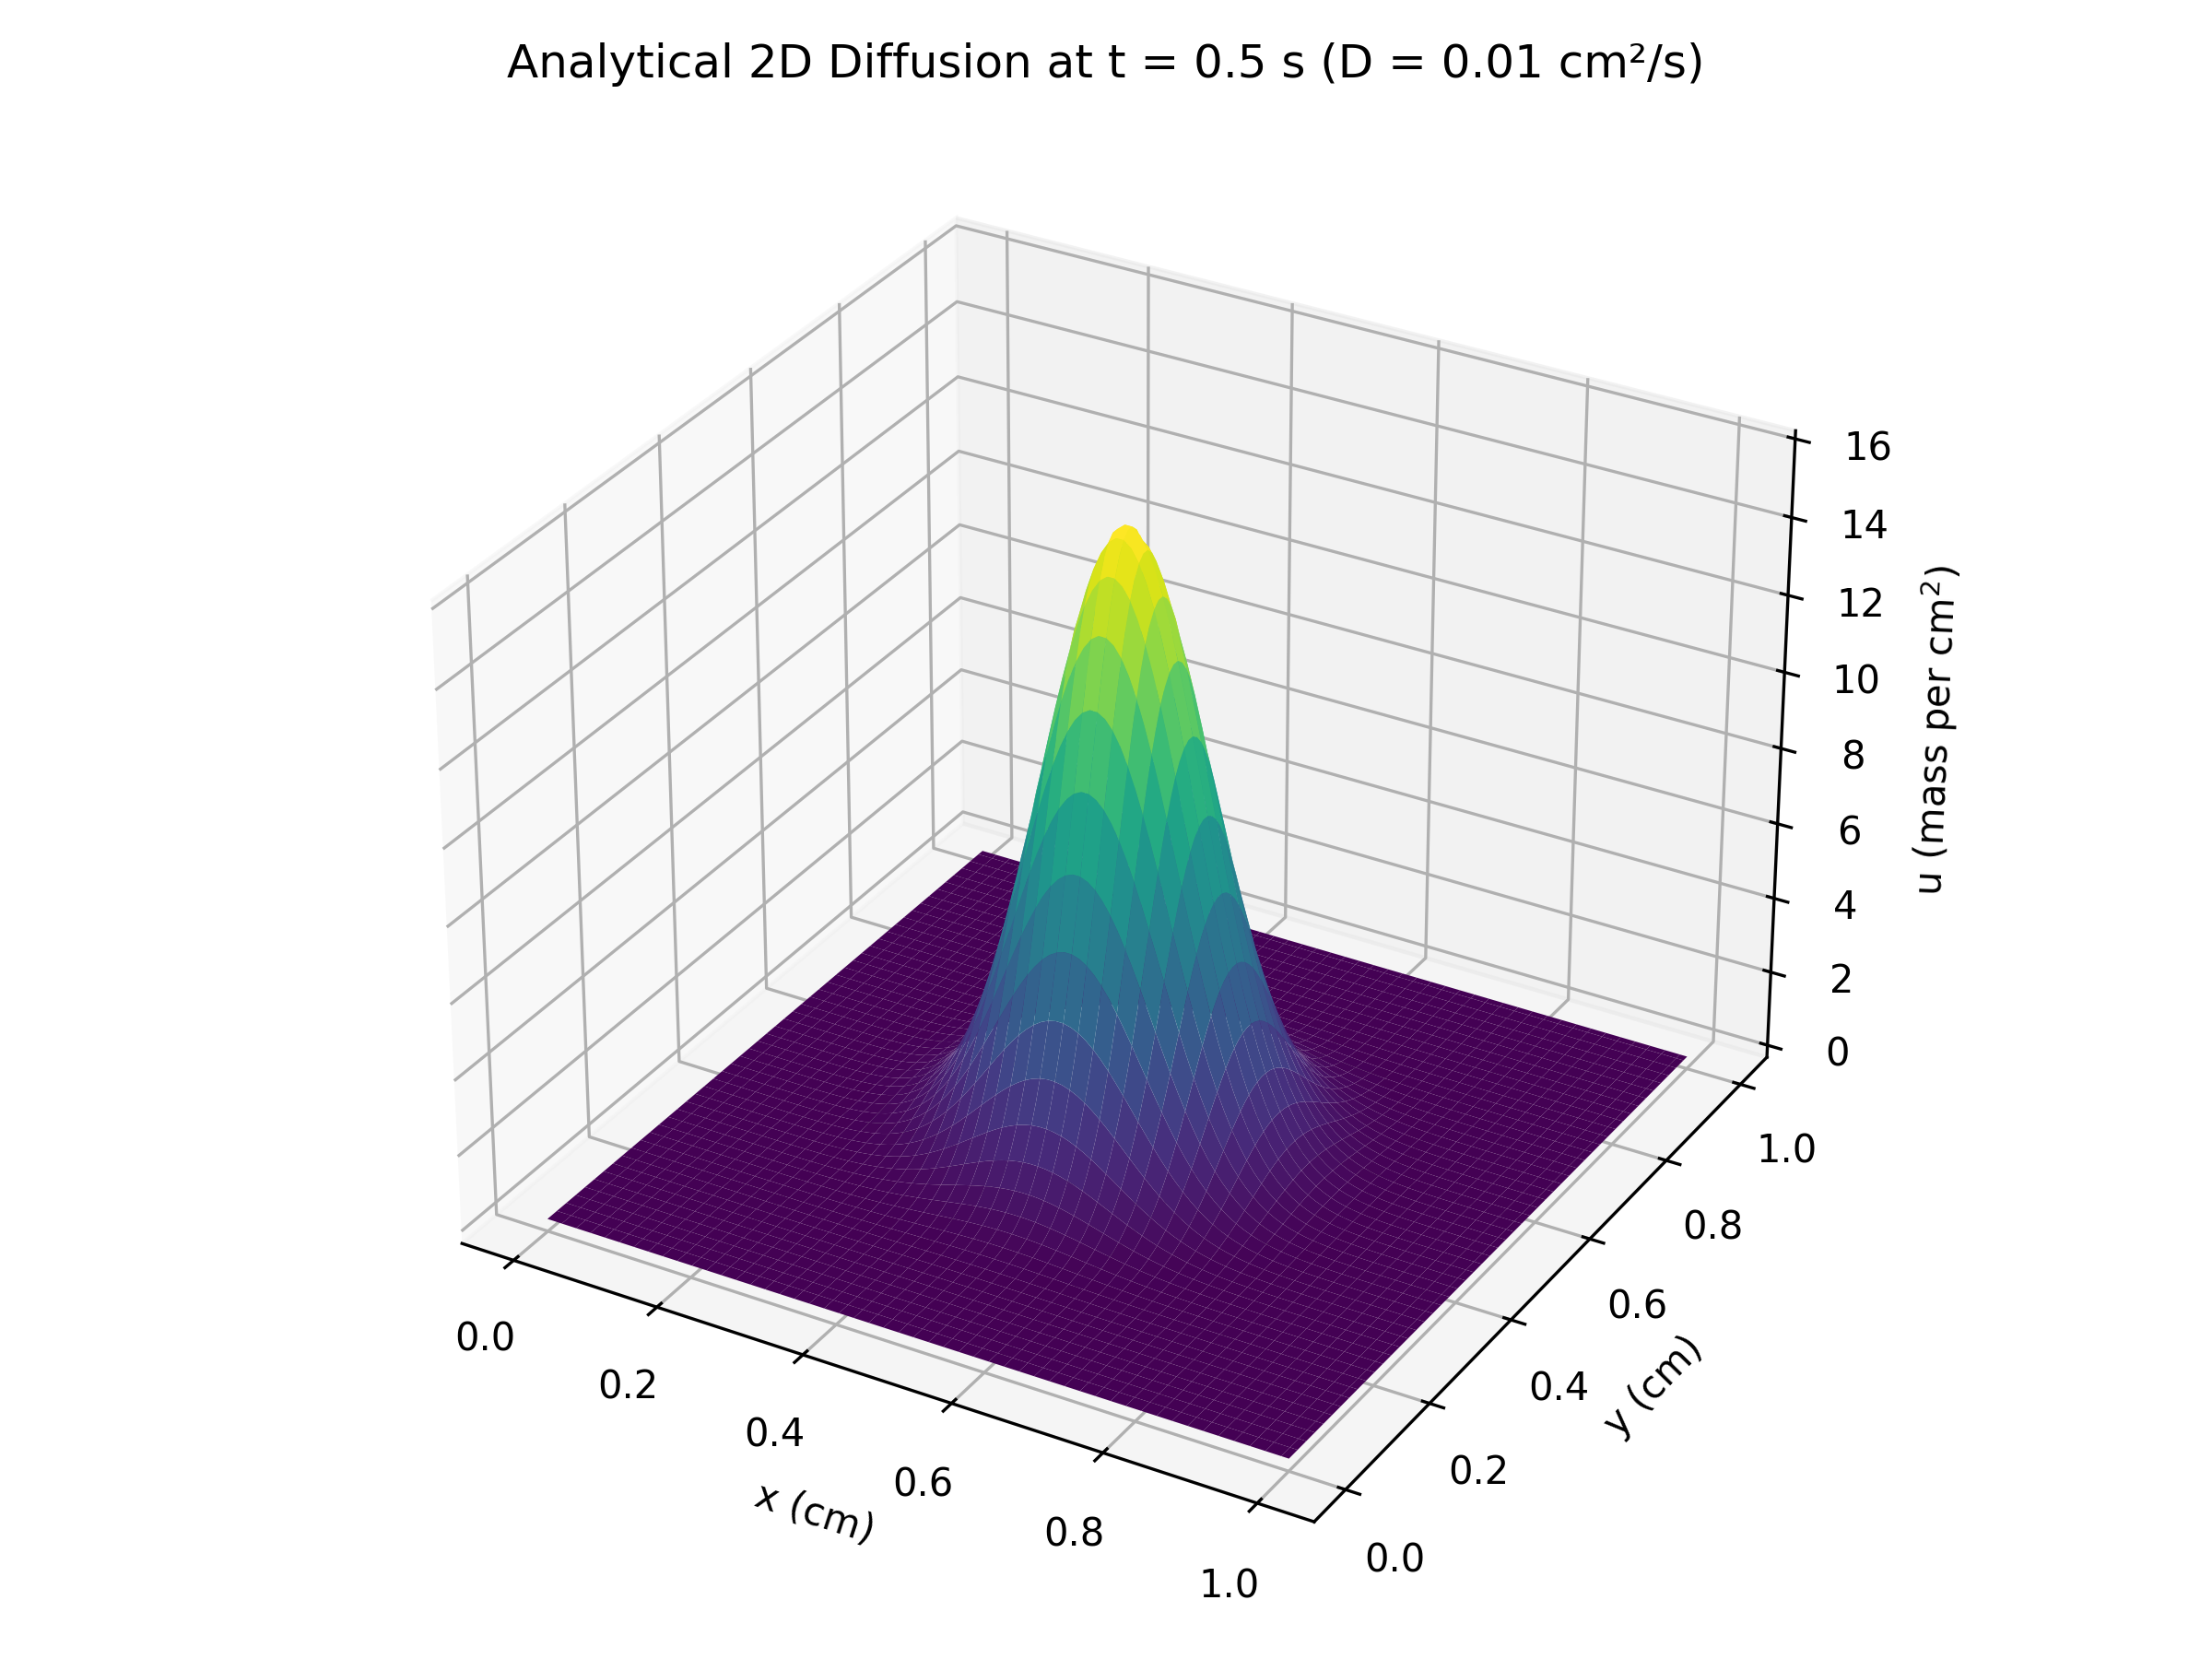
\includegraphics[width=0.6\textwidth]{resources/figures/analytical_solution.png}
  \caption{Analytical solution of 2D diffusion from a point source at \( t = 0.05 \).}
  \label{fig:analytical}
\end{figure}
% --- End replacement ---

\subsection{Physical Interpretation of the Solution}
The analytical solution shows that the drug starts at a single point and spreads out evenly in all directions. The total amount of drug remains constant over time (mass conservation), but the concentration at each point decreases as it spreads.

In real tissues, the diffusion may not be symmetric due to structural anisotropy. In such cases, the solution becomes elongated in the direction where diffusion is faster. Also, if the drug is absorbed or metabolized, the concentration decreases faster over time.

Understanding this behavior helps us predict how far and how fast a drug will spread from the injection point. It also helps in estimating how long it will take for the drug to reach a therapeutic concentration at the target location.

\section{Model and Simulation Structure}

The Python code developed for this project is organized into reusable functions to simulate drug diffusion in various conditions. The core function \texttt{run\_simulation(D\_x, D\_y, lambda\_decay, label)} takes physical parameters and stores the results in structured folders. The output includes heatmaps of drug concentration and animated GIFs for visualization.

The output of each simulation is stored in the \texttt{resources/} directory with a subdirectory named after each case (e.g., \texttt{isotropic\_no\_reaction}). Each of these folders contains:
\begin{itemize}
  \item \texttt{photos/}: a set of PNG images of the concentration field at regular intervals,
  \item an animated file (\texttt{*.gif}) showing the full evolution of the diffusion process.
\end{itemize}

This structure makes it easy to explore the results and compare different physical scenarios.

\section{Numerical Implementation}

\subsection{Choice of Numerical Method}
To simulate the diffusion of a drug in biological tissue, we use the \textbf{finite difference method} (FDM). This method is simple to implement and gives good results for solving partial differential equations. It replaces derivatives with approximations based on values at grid points in space and time.

We apply this method to the 2D diffusion-reaction equation. The time derivative is solved using the \textbf{Forward Euler method}, which is an explicit time-stepping scheme. Even though this method is conditionally stable, it is easy to code and works well with small time steps.

This approach lets us simulate both \textbf{isotropic} diffusion (same rate in all directions) and \textbf{anisotropic} diffusion (different rates in different directions). We can also include a \textbf{reaction term} to simulate how the drug is absorbed or breaks down inside the tissue.

\subsection{Description of the Numerical Scheme}
We define a square simulation domain divided into a grid of \( N \times N \) points. Let \( \Delta x \) and \( \Delta y \) be the spatial steps (usually the same), and \( \Delta t \) be the time step.

Let \( u_{i,j}^n \) be the approximation of the drug concentration \( u(x, y, t) \) at grid point \( (i,j) \) and time step \( n \). The finite difference update rule for the diffusion equation with anisotropic diffusion and a linear reaction is:

\[
u_{i,j}^{n+1} = u_{i,j}^n + \Delta t \left[ D_x \frac{u_{i+1,j}^n - 2u_{i,j}^n + u_{i-1,j}^n}{\Delta x^2} + D_y \frac{u_{i,j+1}^n - 2u_{i,j}^n + u_{i,j-1}^n}{\Delta y^2} - \lambda u_{i,j}^n \right]
\]

We use \textbf{homogeneous Neumann boundary conditions}, meaning the gradient of \( u \) at the edges is zero. This condition represents a tissue where the drug cannot escape the domain.

The \textbf{initial condition} is a 2D Gaussian centered in the grid, simulating a local injection of the drug.

\subsection{Stability and Convergence Analysis}
Since we use the \textbf{explicit Forward Euler method}, stability is a key concern. The method is stable only if the time step \( \Delta t \) satisfies the \textbf{Courant–Friedrichs–Lewy (CFL)} condition:

\[
\Delta t \leq \frac{1}{2} \left( \frac{1}{D_x / \Delta x^2 + D_y / \Delta y^2} \right)
\]

If this condition is not respected, the solution may diverge or show unphysical oscillations.

To check convergence, we can repeat the simulation with smaller time and space steps and compare the results. If the method is converging, the numerical error should decrease as we refine the grid. In practice, we measure the difference between successive solutions and verify that the error decreases as expected.

\subsection{Test Case Simulation}
We test the numerical scheme on a 2D domain of size 1 cm × 1 cm, discretized into a 100 × 100 grid. The initial drug concentration is defined by:

\[
u(x, y, 0) = \exp\left( -\frac{(x - 0.5)^2 + (y - 0.5)^2}{2\sigma^2} \right)
\]

with \( \sigma = 0.05 \), creating a Gaussian peak at the center of the domain.

We perform simulations with:
\begin{itemize}
    \item \( D_x = D_y = 0.01 \) cm\(^2\)/s (isotropic case),
    \item \( D_x = 0.01 \), \( D_y = 0.001 \) (anisotropic case),
    \item with and without a reaction rate \( \lambda = 0.1 \).
\end{itemize}

The simulation runs for a total time of 1 second, with a time step satisfying the stability condition. At each step, we save the solution to observe the drug spreading.

In the next section, we present heatmaps and line plots showing the differences between isotropic and anisotropic diffusion, as well as the effect of the reaction term.

\subsection{Python Code Example}

Below is a simplified version of the Python function used to perform the simulations:

\begin{lstlisting}[language=Python, caption=Core simulation loop in Python]
def run_simulation(D_x, D_y, lambda_decay, label):
    dt = 0.25 * min(dx**2 / D_x, dy**2 / D_y)
    Nt = int(T / dt)
    u = np.exp(-((X - 0.5)**2 + (Y - 0.5)**2) / (2 * sigma**2))
    ...
    # Update scheme, boundary conditions, saving plots and animations
\end{lstlisting}

\section{Results and Visualizations}

\subsection{Isotropic vs Anisotropic Diffusion Comparison}
To better understand the effects of anisotropy, we compare two simulations: one with isotropic diffusion (\( D_x = D_y \)) and one with anisotropic diffusion (\( D_x \neq D_y \)). In the isotropic case, the drug spreads symmetrically in all directions, creating a circular concentration profile. In contrast, the anisotropic case produces an elliptical pattern, where the drug moves faster in the direction with the higher diffusion coefficient.

For example, when \( D_x = 0.01 \) and \( D_y = 0.001 \), the drug spreads more along the \( x \)-axis and less along the \( y \)-axis. This kind of behavior is realistic in biological tissues such as muscles or nerves, where the structure can guide diffusion in one direction more than others.

\begin{figure}[h!]
  \centering
  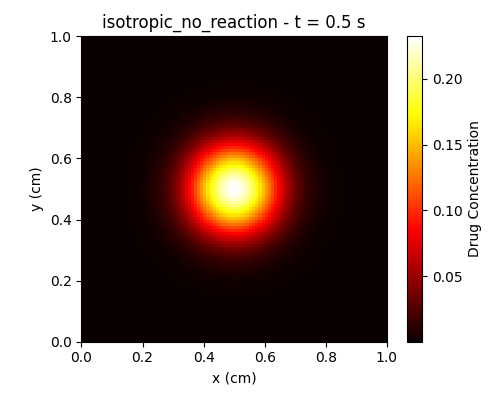
\includegraphics[width=0.7\textwidth]{resources/isotropic_no_reaction/photos/diffusion_5.png}
  \caption{Isotropic diffusion at intermediate time step.}
  \label{fig:isotropic}
\end{figure}

\begin{figure}[h!]
  \centering
  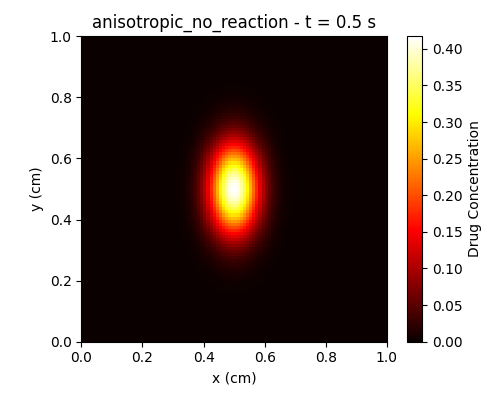
\includegraphics[width=0.7\textwidth]{resources/anisotropic_no_reaction/photos/diffusion_5.png}
  \caption{Anisotropic diffusion at same time step (note the elongated shape).}
  \label{fig:anisotropic}
\end{figure}

\subsection{Concentration Curves and Maps}
We visualize the drug concentration using 2D heatmaps and 1D cross-sectional plots. Heatmaps show how the drug concentration evolves over time on the full 2D domain, while 1D plots (for example, along the horizontal center line \( y = 0.5 \)) give us a clearer view of the concentration profile.

In the isotropic case, the heatmaps show smooth, circular diffusion patterns. In the anisotropic case, the shape becomes stretched, confirming that the drug moves faster in one direction.

We also plot the maximum concentration over time. In both cases, the peak concentration decreases as the drug spreads, but it decreases faster in the anisotropic case because the drug spreads more quickly in at least one direction.

\subsection{Validation Using Analytical Solution}
To validate our numerical method, we compare it to the analytical solution of the isotropic diffusion equation without a reaction term. The analytical solution is a 2D Gaussian:

\[
u(x, y, t) = \frac{1}{4 \pi D t} \exp\left(-\frac{(x - x_0)^2 + (y - y_0)^2}{4 D t} \right)
\]

We compute the numerical error by subtracting the analytical solution from the numerical one at selected time steps. We then calculate the root-mean-square error (RMSE) over the grid. When the time step is small enough, and the CFL condition is satisfied, the error remains small and confirms the accuracy of the simulation.
In our test, the numerical simulation had a peak concentration of approximately 0.15 mass/cm², distributed over an area of about 0.8 cm².
The analytical solution for the same parameters predicted a similar shape and maximum value. However, the root-mean-square error (RMSE) at \( t = 1.0 \) s was measured at 1.95 mass/cm², which is significantly higher than the expected average values. This suggests that the numerical scheme introduces non-negligible errors, likely due to resolution limitations or imperfect normalization.
Future refinements with a finer grid or smaller time steps are expected to reduce this discrepancy and improve agreement with the analytical model.

This comparison gives us confidence that the finite difference method correctly captures the diffusion behavior, especially in the isotropic case. For anisotropic cases, where no simple analytical solution exists, we rely on physical interpretation and visual consistency.

\section{Conclusion}

\subsection{Summary of Results}
In this project, we studied the diffusion of a drug in biological tissues using both analytical and numerical approaches.
We started with a review of the physical and mathematical background of the diffusion equation, focusing on its application to drug delivery problems.

We then analyzed the properties of the equation and solved a simplified version analytically.
This gave us useful insights into how the drug spreads over time in an idealized situation.
After that, we developed a numerical scheme based on the finite difference method to simulate the diffusion process, including anisotropic effects and a possible reaction term.

Our simulations showed how anisotropy affects the drug’s spread and how the reaction term can accelerate the decrease in concentration.
We also validated our numerical results against the analytical solution in the isotropic case, and the errors were small, which confirms that our implementation is correct.

\subsection{Limitations and Future Improvements}
There are a few limitations in our current model. First, we only used a 2D rectangular domain with simple geometry.
Real tissues can have complex shapes, varying properties, and moving boundaries.
Second, we used constant diffusion coefficients, while in practice, they may vary with position or even depend on the concentration.
Third, the reaction term was linear and simple, but real biological reactions are often nonlinear and more complex.

In future work, we could improve the model by:
\begin{itemize}
    \item using finite element methods to simulate more realistic tissue geometries,
    \item implementing spatially varying or nonlinear diffusion and reaction terms,
    \item coupling the model with blood flow (convection-diffusion),
    \item and validating the results with real experimental or medical data.
\end{itemize}

Despite these simplifications, this project shows how partial differential equations can help us understand and predict the behavior of drug diffusion in tissues.
The combination of mathematical analysis and numerical simulation gives useful tools to study biomedical problems.

\begin{thebibliography}{9}
\bibitem{pmc1} https://www.ncbi.nlm.nih.gov/pmc/articles/PMC5763252/
\bibitem{pmc2} https://www.ncbi.nlm.nih.gov/pmc/articles/PMC7491225/
\bibitem{sciencedirect} https://www.sciencedirect.com/
\bibitem{springer} https://link.springer.com/
\bibitem{pubmed} https://pubmed.ncbi.nlm.nih.gov/
\bibitem{wikipedia} https://en.wikipedia.org/wiki/Diffusion
\end{thebibliography}

\end{document}